
	\chapter{Der kosmische Mikrowellenhintergrund\label{chapter:thema}}
	\lhead{Der kosmische Mikrowellenhintergrund}
	\begin{refsection}
		\chapterauthor{Hansruedi Patzen und Nico Vinzens}
		
		\printbibliography[heading=subbibliography]
	\end{refsection}
	\section{Einleitung}
	Ähnlich wie der Lebensraum der Fische auf das Wasser begrenzt ist, so ist unser Lebensraum begrenzt auf das Universum.
	Weiss ein Fisch, wie das Meer von unserem Blickpunkt aus aussieht?
	Wahrscheinlich nicht, wieso sollte ihn das auch interessieren?
	Da wir aber keine Fische sind, ist es nur natürlich sich zu fragen, wie das Universum von Aussen betrachtet, aussieht.
	Um die Frage nach der Form des Universums beantworten zu können, werden wir uns im folgenden Kapitel mit dem kosmischen Mikrowellenhintergrund befassen.
	
	\subsection{Der komische Mikrowellenhintergrund}
	Glaubt man der Theorie des Big-Bang, (was wir im folgenden tun wollen) so waren der Druck und die Temperaturen in den ersten ca. 380'000 Jahren nach dem Big-Bang so, dass Atome nicht existieren konnten.
	Die gesamte Masse bestand stattdessen aus ionisiertem Plasma, welches sehr effizient darin war, Strahlung zu zerstreuen (dieser Effekt ist unter Thomson-Streuung bekannt).
	Dadurch ist es Forschern heute unmöglich, nachzuvollziehen, was in dieser Zeit passiert ist.
	Alles versteckt sich hinter einer Art undurchdringlichen Nebels (siehe Abbildung \ref{fig:radiation_scattering}).
	\begin{figure}
		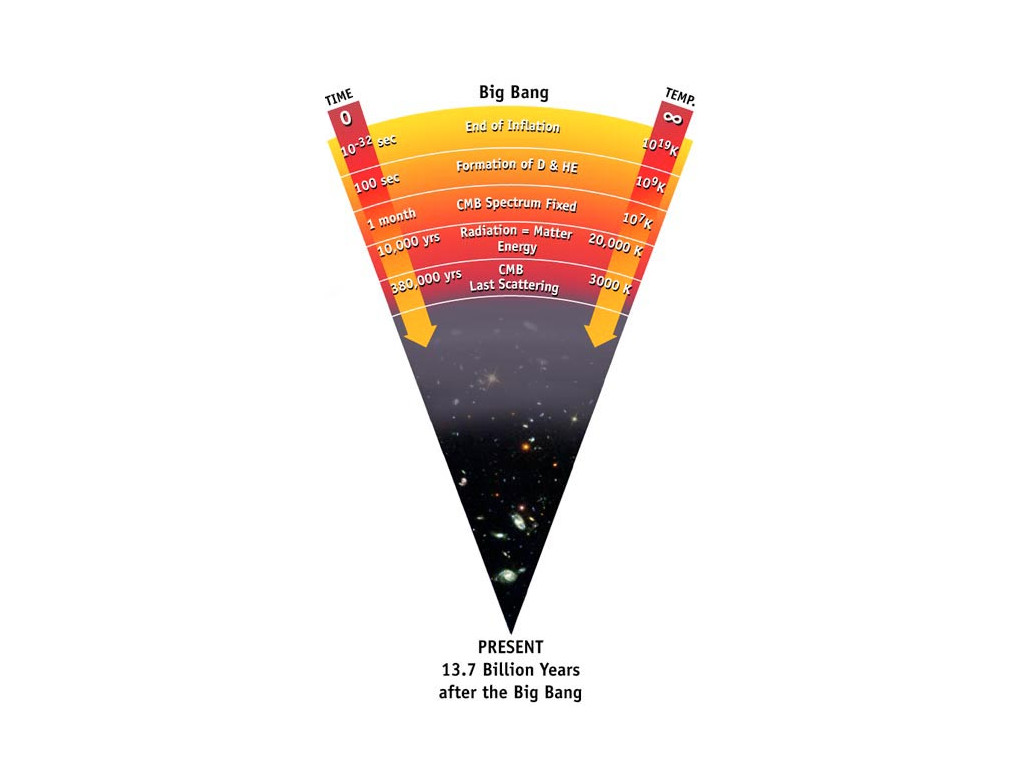
\includegraphics[scale=1]{cmb/images/radiation_scattering.jpg}
		\caption{Sichtbarkeit des Universums im Zeitverlauf}
		\label{fig:radiation_scattering}
	\end{figure}
	Im Verlauf der nächsten 380'000 Jahre und der damit verbundenen Ausdehnung des Universums sanken Druck und damit die Temperatur stark, nämlich auf 3.000 Kelvin.
	Dies entspricht der Temperatur einer Schwarzkörperstrahlung, Strahlung von einem Schwarzen Körper, welcher Strahlung absorbiert und nicht wieder rauslässt (Dieser Fakt ist essentiell zur spätern Nachweisung der kosmischen Hintergrundstrahlung).
	Nun waren die Bedingungen erfüllt, dass sich Protonen und Elektronen zu Wasserstoffatomen verbinden konnten.
	Man spricht hier von Rekombination.
	Nach dieser Rekombinaton gab es keine freien Elektronen mehr, wodurch die Photonen nicht mehr durch Thomson-Streuung abgelenkt wurden.
	Den Photonen war es jetzt endlich möglich, dem Nebel des jungen Universums zu entkommen und sich frei zu bewegen.
	Die kosmische Hintergrundstrahlung ist eine Aufzeichnung der Photonen zum Zeitpunkt der Rekombination.
	\ref{CMB_intro}
	
	\subsection{Die Entdeckung des kosmischen Mikrowellenhintergrunds}
	Nachdem bereits zahlreiche Forscher erfolglos nach dem kosmischen Mikrowellenhintergrund gesucht hatten, geschah die tatsächliche Entdeckung der Strahlung, wie so oft in der Wissenschaft, per Zufall.
	Im Jahr 1964 arbeiteten Arno Penzias und Robert Woodrow Wilson an einer sogenannten "Large Horn Antenna" (siehe Abbildung \ref{fig:wilson_penzias}).
	\begin{figure}
		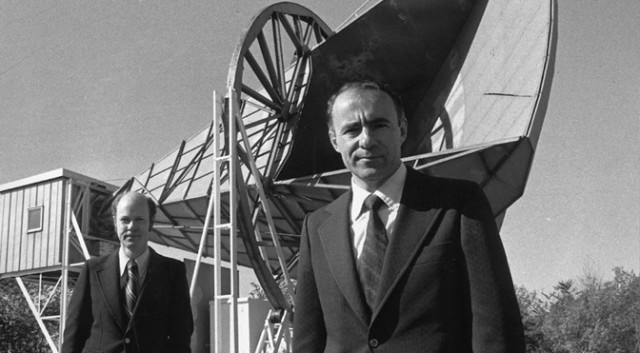
\includegraphics[scale=1]{cmb/images/penzias-wilson-large-horn-antenna.jpg}
		\caption{Robert W. Wilson (links) und Arno A. Penzias vor ihrer Antenne}
		\label{fig:wilson_penzias}
	\end{figure}
	Dabei fanden sie ein Störsignal, welches unabhängig von der Ausrichtung der Antenne gleich war.
	Auch eine Reinigung der Antenne brachte keine Verbesserung, weshalb sie sich an andere Physiker wandten, welche bestätigten, dass es sich beim Störsignal um die erste Aufzeichnung der kosmischen Hintergrundstrahlung handelte.
	Der Fund gilt als eine der wichtigsten Entdeckungen der Kosmologie und als Bestätigung der Urknalltheorie.
	Deswegen wurde ihnen dafür 1978 der Nobelpreis für Physik verliehen.
	
	In den Messungen von Wilson und Penzias wurde eine extreme Isotropie in der Strahlung festgestellt.
	Dies stellte ein Problem dar, da dass heutige Universum sich nur gebildet haben kann, wenn auch im Universum vor der Rekombination bereits Dichteschwankungen existiert haben.
	Diese Schwankungen müssten auch in Temperaturunterschieden der kosmischen Hintergrundstrahlung erkennbar sein.
	Fast 30 jahre lang (1965-1992) blieb die Suche nach diesen Anisotropien erfolglos.
	In dieser Zeit bemerkte man, dass die Temperaturschwankungen innerhalb des Strahlung extrem klein sein muss (< 0.001 Prozent).
	Die Erlösung brachte 1992 schliesslich der COBE Satellit.
	\ref{m_schönitzer}
	
	\subsection{COBE}
	Die COBE (Cosmic Background Explorer) Mission, hatte den Zweck, exakte Messungen der kosmischen Infrarot-(hier nicht näher behandelt) und Hintergrundstrahlung durchzuführen.
	Der Satellist wurde am 18. November 1989 ins all geschossen und verfügte über drei Messinstrumente:
	\begin{itemize}
		\item DIRBE (Diffuse Infrared Background Experiment): Um nach der kosmischen Infrarotstrahlung zu suchen.
		Dank der Messung dieser Strahlung konnten unter anderem Modelle der Entstehung von Sternen erstellt werden.
		\item DMR (Differential Microwave Radiometer): Um die Anisotropie der kosmischen Hintergrundstrahlung nachzuweisen.
		\item FIRAS (Far Infrared Absolute Spectrophotometer): Um die Temperatur der kosmischen Hintergrundstrahlung nachzuweisen. 
	\end{itemize}
	\ref{COBE}
	Das Resultat dieser Messungen ist in Abbildung \ref{fig:COBE} zu sehen.
	\begin{figure}
		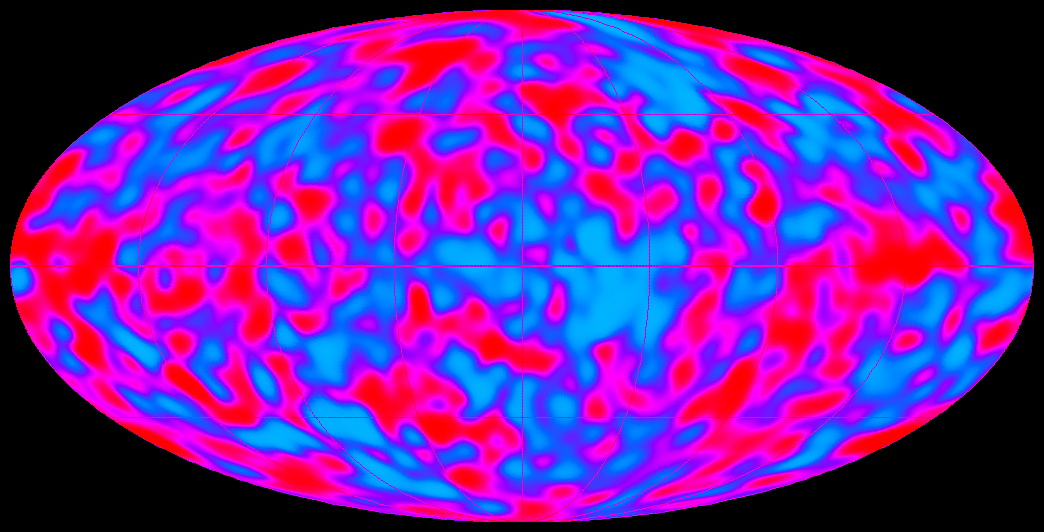
\includegraphics[scale=1]{cmb/images/COBE_CMB.jpg}
		\caption{Das erste Bild der kosmischen Hintergrundstrahlung}
		\label{fig:COBE}
	\end{figure}
	Die COBE Mission war ein voller Erfolg.
	Die letzten Zweifel an der Urknall-Theorie konnten zerstreut werden
	DMR konnte Temperaturschwankungen zwischen verschiedenen Stellen am Himmel von 10^-5 nachweisen, womit die Anisotropie der Strahlung bewiesen war.
	FIRAS mass den spektralen Verlauf der Strahlung und kam zum Ergebnis, dass ihre Temperatur extrem genau der eines Schwarzkörpers entspricht, nämlich 2.725 K (siehe Abbildung \ref{fig:CMB_spectrum}).
	Damit war bewiesen, dass es sich bei der gemessen Strahlung tatsächlich um die kosmische Hintergrundstrahlung handelt, da man weiss, dass eine zur Rekombination entstandene Schwarzkörperstrahlung sich von 3 K auf eben diese 2.725 K abgekühlt haben muss.
	
	John C. Mather (NASA) und George F. Smoot (University of California), erhielten für ihre Arbeit an der COBE Mission 2006 den Nobel Preis für Physik.
	\begin{figure}
		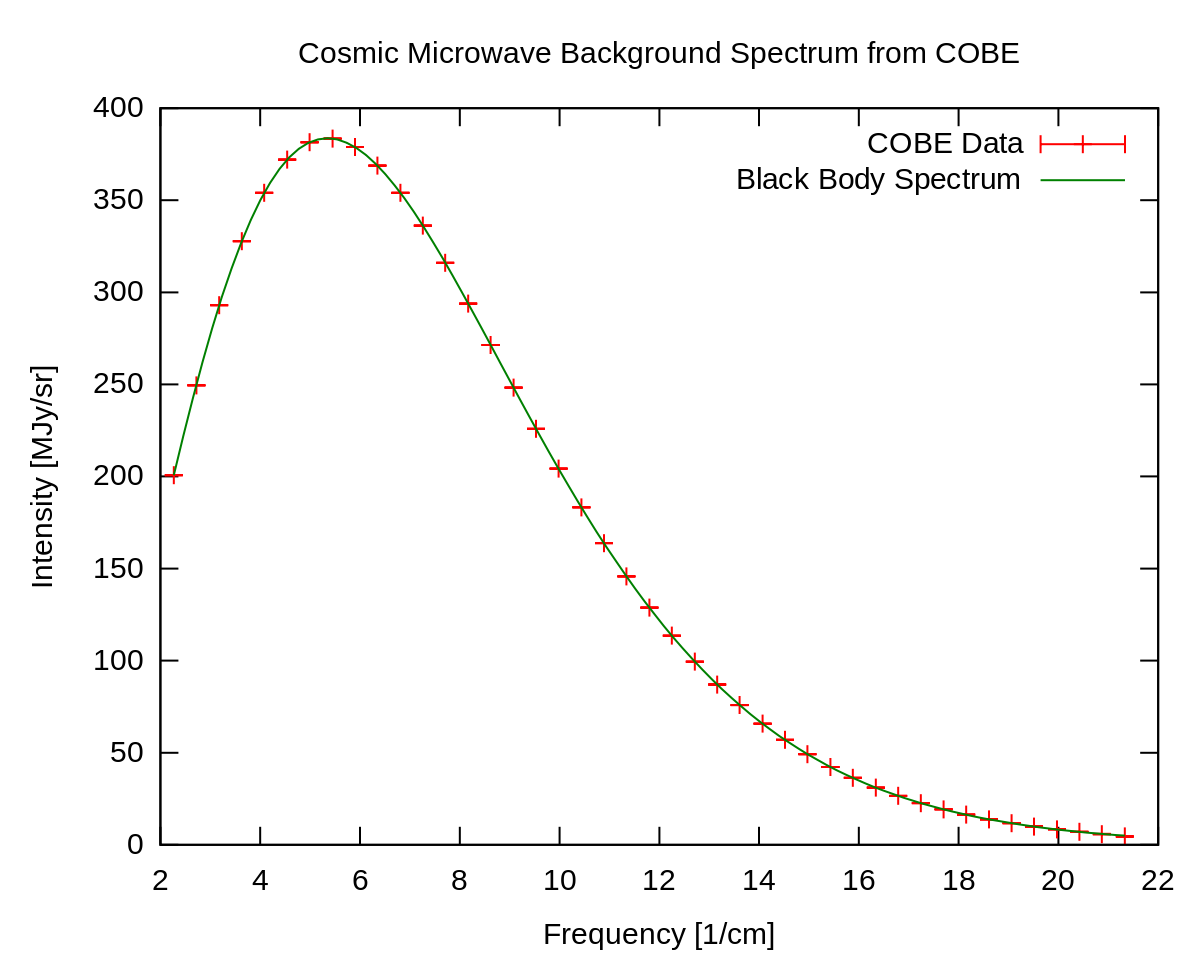
\includegraphics[scale=1]{cmb/images/CMB_spectrum.png}
		\caption{Das von COBE gemessene Spektrum stimmt perfekt mit dem erwarteten Schwarzkörper-Spektrum überein.}
		\label{fig:CMB_spectrum}
	\end{figure}
	
	\subsection{WMAP und Planck}
	WMAP (NASA) und Planck (ESA, European Space Agency) folgten auf COBE.
	Ihr Ziel war es unter anderem, präzisere Bilder der kosmischen Mikrowellenhintergrundstrahlung zu erhalten.
	\subsubsection{WMAP (Wilkinson Microwave Anisotrophy Probe)}
	WMAP wurde im Juni 2001 ins All geschossen, mit dem Ziel verschiedenste kosmologische Messungen durchzuführen.
	Die Resultate dieser Messungen sind sehr vielfältig, deswegen werden die interessantesten hier kurz aufgeführt:
	\begin{itemize}
		\item Messung der kosmischen Hintergrundstrahlung: Durch die WMAP Messungen konnte ein sehr exaktes Bild der Strahlung erzeugt werden (siehe Abbildung \ref{fig:CMB_WMAP}).
		\begin{figure}
			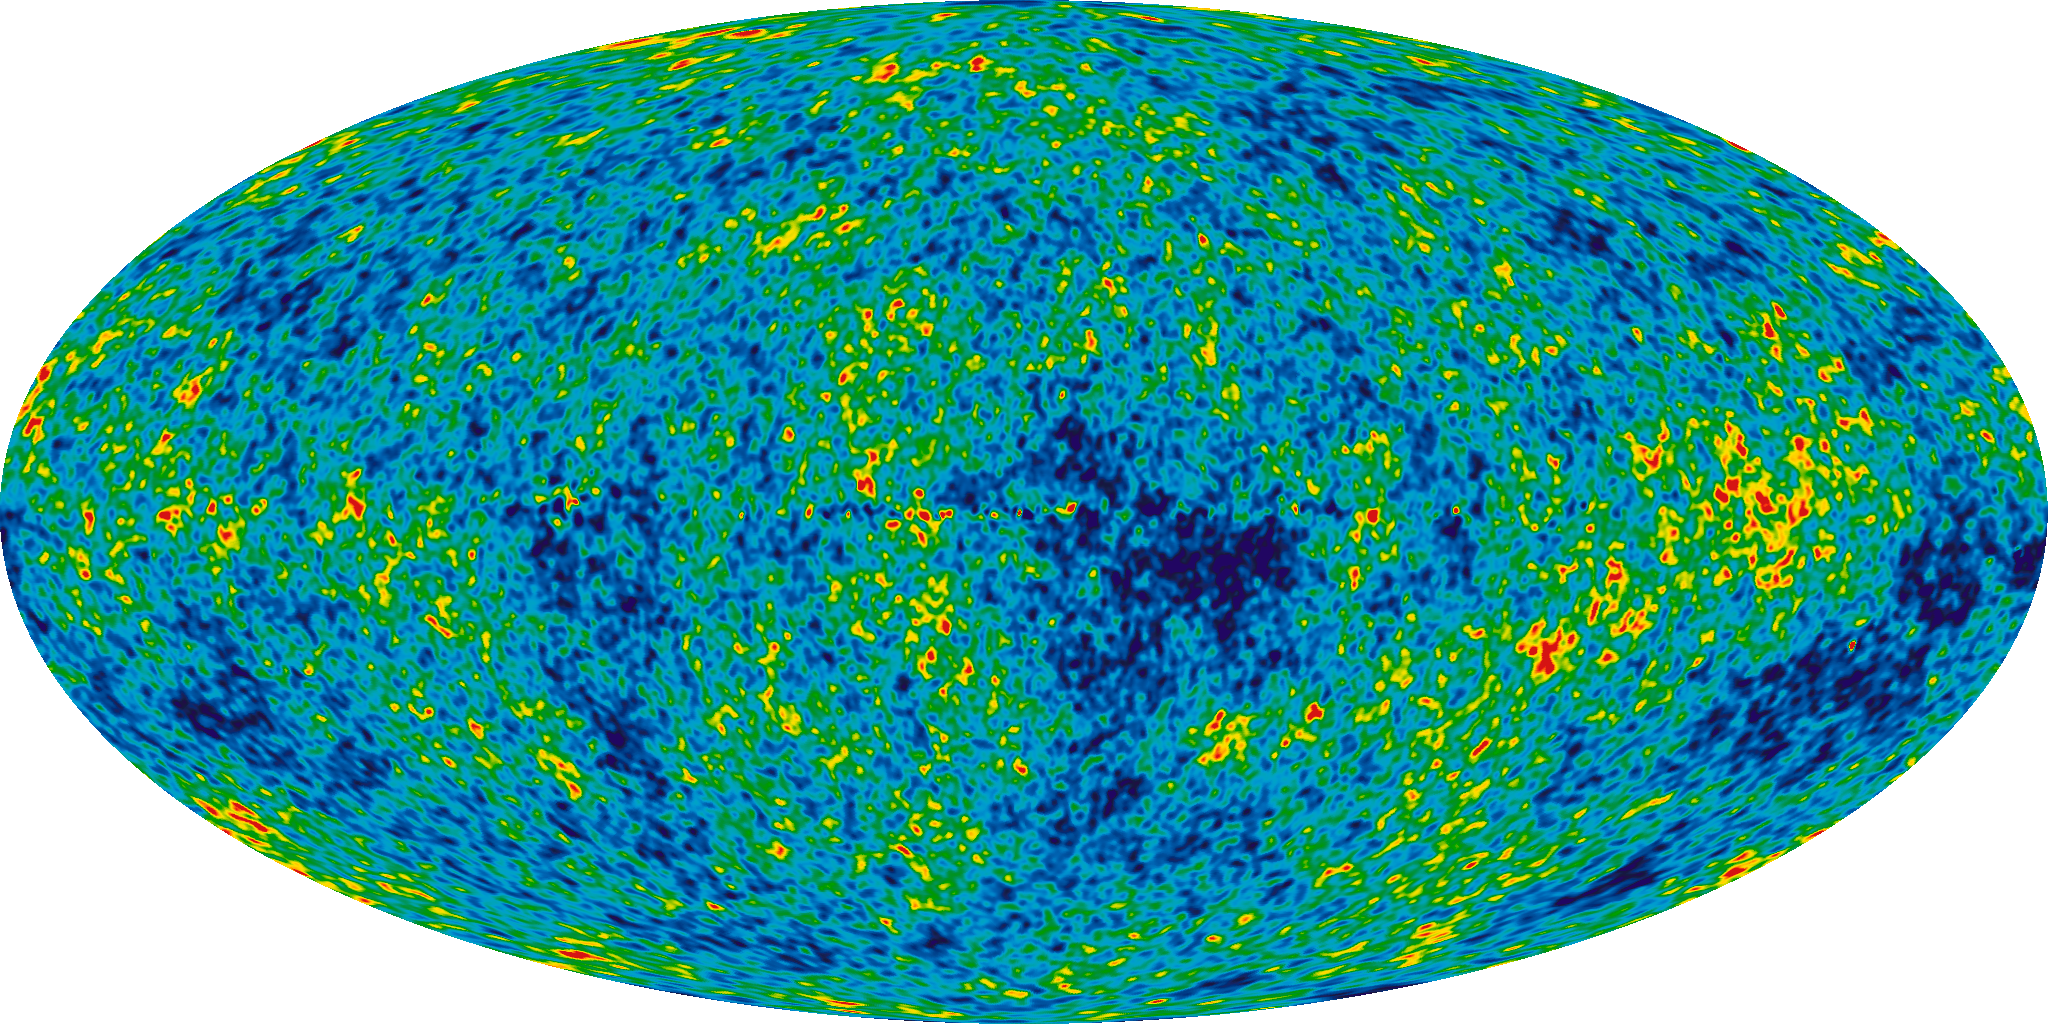
\includegraphics[scale=1]{cmb/images/CMB_WMAP.png}
			\caption{Kosmischer Mikrowellenhintergrund gemessen von WMAP}
			\label{fig:CMB_WMAP}
		\end{figure}
		\item Alter des Universums: Das Alter des Universums konnte auf ein halbes Prozent genau auf 13.77 Milliarden Jahre bestimmt werden
		\item Dunkle Materie und dunkle Energie: Es konnte bestimmt werden, dass das Universum zu 24.0 Prozent aus dunkler Materie und zu 71.4 Prozent aus dunkler Energie besteht.
	\end{itemize}
	Dies ist ist nur ein kleiner Ausschnitt aus den vielfältigen Resultaten der WMAP Mission.
	\ref{CMB_WMAP}
	
	\subsubsection{Planck}
	Planck wurde 2009 abgeschossen, um die kosmische Mikrowellenhintergrundstrahlung noch genauer als bisher studieren zu können.
	Das Ziel war es das derzeitige Standardmodell des Universums so zu bestätigen, dass es über jeden Zweifel erhaben ist.
	Aus den Daten konnte folgendes Bild generiert werden:
	\begin{figure}
		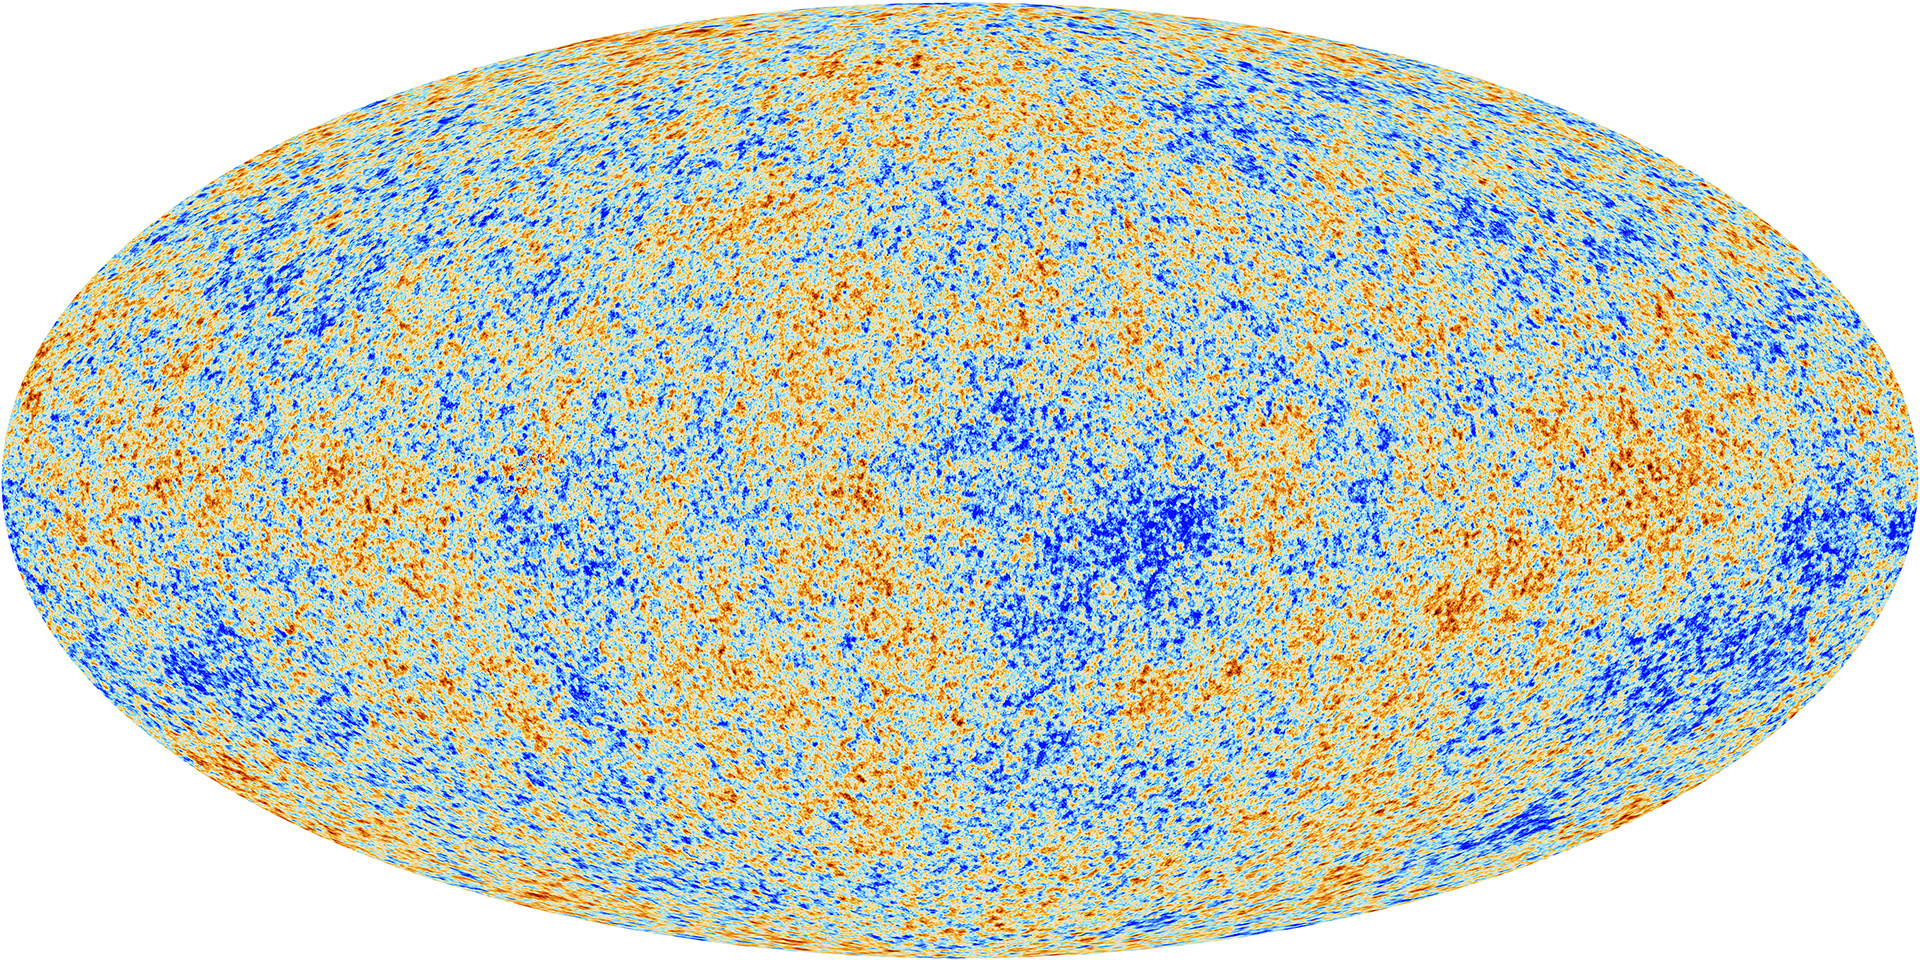
\includegraphics[scale=1]{cmb/images/CMB_Planck.jpg}
		\caption{Kosmischer Mikrowellenhintergrund gemessen von Planck}
		\label{fig:CMB_Planck}
	\end{figure}
	Das Ziel von Planck wurde erreicht und das zurzeit anerkannte Modell konnte bestätigt werden.
	
	\subsection{Vergleich}
	Mit dem folgenden Bild können die Genauigkeitsunterschiede im direkten Vergleich gut dargestellt werden:
	\begin{figure}
		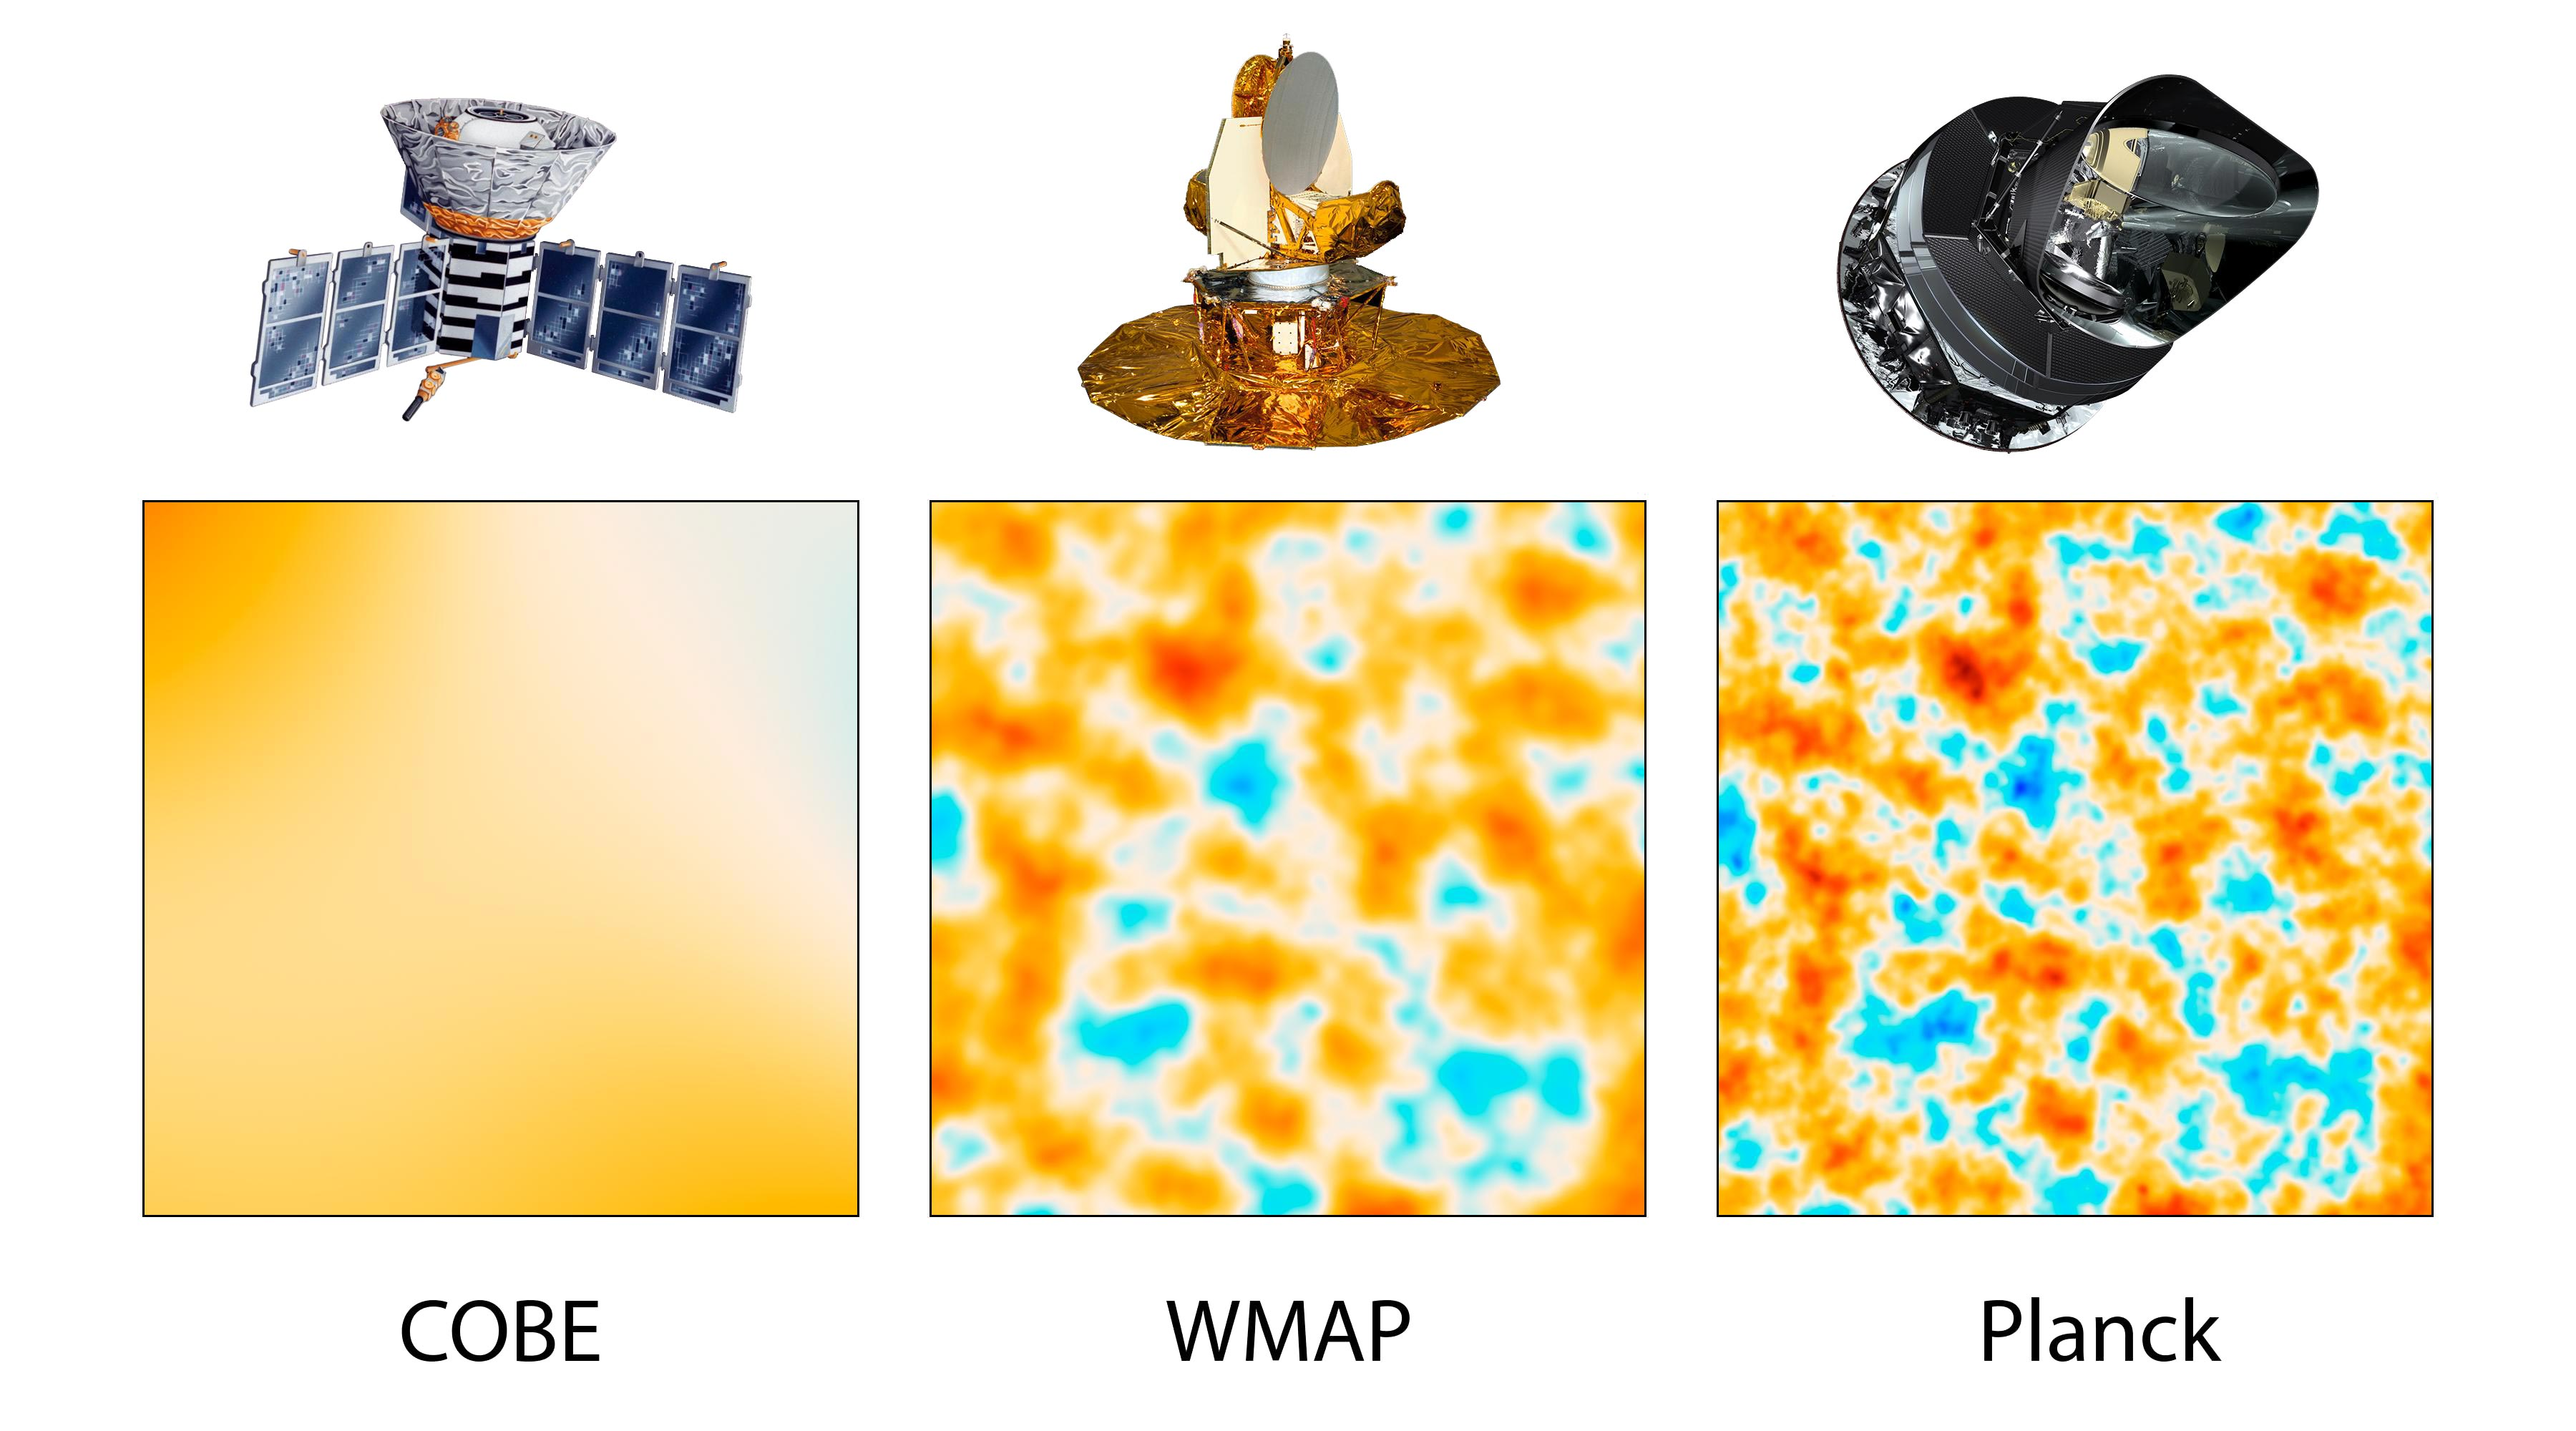
\includegraphics[scale=1]{cmb/images/COBE_WMAP_Planck.jpg}
		\caption{Direkter Vergleich der aus den verschiedenen Missionen entstandenen Bildern}
		\label{fig:COBE_WMAP_PLANCK}
	\end{figure}
	Wie man sieht, sind die Verbesserungen beträchtlich.
	Das Bild von Planck dient auch als Grundlage für die Berechnungen, die später noch aufgezeigt werden.
	
	
	\subsection{Die Formen des Universums}
	Eine der spannendsten Fragen der Kosmologie ist eine ganz simple: Welche Form hat unser Universum?
	
	Nach der Entdeckung und Messung der kosmischen Mikrowellenhintergrundstrahlung ist es uns möglich, diese Frage zu beantworten.
	Die Frage nach der Form eines Körpers ist überraschend einfach durch die klassische Geometrie zu klären.
	Grundsätzlich sind drei mögliche Formen denkbar:
	\begin{itemize}
		\item Das Universum könnte positiv gekrümmt sein, wie eine Kugel.
		Zwei parallele Linien auf der Kugeloberfläche kreuzen sich und die Winkelsumme eines Dreiecks ist grösser als 360 Grad.
		\item Das Universum könnte negativ gekrümmt sein, wie ein Sattel.
		Zwei parallele Linien weichen immer stärker voneinander ab und die Winkelsumme eines Dreiecks ist kleiner als 360 Grad.
		\item Das Universum könnte flach sein, wie ein Blatt Papier.
		Zwei parallele Linien berühren sich nie und die Winkelsumme eines Dreiecks beträgt 360 Grad.
	\end{itemize}
	Dieses Konzept lässt sich auch auf unser Universum übertragen.
	Da es uns möglich ist in der Zeit zurückzublicken, können wir die Bilder aus der Vergangenheit analysieren und so auf die Form des Universums schliessen.
	Wir wissen welche Temperatur die kosmische Mikrowellenhintergrundstrahlung zum Zeitpunkt der Rekombination gehabt haben muss (durch zurückrechnen).
	Dann können die aufgenommenen Bilder der Strahlung als Vergleich herebeiziehen:
	\begin{itemize}
		\item Ist das Universum positiv gekrümmt, wäre ein Vergrösserungseffekt festzustellen.
		Die Temperatur würde bei uns höher erscheinen? als sie es wirklich ist.
		\item Ist das Universum negativ gekrümmt, wäre ein Verkleinerungseffekt festzustellen.
		Die Temperatur würde bei uns tiefer erscheinen, als sie es wirklich ist.
		\item Ist das Universum flach, würde die Temperatur genau so sein, wie berechnet.
	\end{itemize} 
	
	
	\section{Berechnungen}

